\documentclass[11pt]{article}

\usepackage[a4paper,margin=1in]{geometry}
\usepackage[T1]{fontenc}
\usepackage{lmodern}
\usepackage{microtype}
\usepackage{booktabs}
\usepackage{array}
\usepackage{xcolor}
\usepackage{hyperref}
\usepackage{tikz}
\usetikzlibrary{arrows.meta,positioning,shapes.geometric}

\hypersetup{
  colorlinks=true,
  linkcolor=blue!55!black,
  urlcolor=blue!55!black,
  citecolor=blue!55!black
}

\title{\textbf{NAGARE}\\Holonomy Learning with Projection-Gated Global Pooling}
\author{Kyberszittya / HyMeKo Research Extraction}
\date{2026-07-02}

\newcommand{\us}{\ensuremath{\mu\mathrm{s}}}
\emergencystretch=2em

\begin{document}
\maketitle

\begin{abstract}
NAGARE is an experimental Rust implementation of local holonomy-based learning
with quaternion periodic features, global pooling, Clifford error metrics, and
projection-gated updates. The current extraction targets small generated
point-set tasks such as moons, spiral, and xor. The strongest current result is
a fitted rank-6 projection gate that improves the difficult spiral
few-shot/noisy/missing stress row while keeping microsecond-scale CPU forward
passes and a small parameter count.
\end{abstract}

\section{Positioning}

NAGARE is not presented as a general replacement for backpropagation. It is a
research artifact for testing whether structured local updates can be useful
when the input is represented through geometry, periodicity, and holonomy.

The repository intentionally reuses HyMeKo primitives where the logic is not
NAGARE-specific. Quaternion rotor operations and Clifford probability error are
provided by \texttt{hymeko\_clifford} through a path dependency during
incubation.

\section{Architecture}

Each generated sample is a small point set. The point set is lifted into
quaternion periodic features, pooled globally, optionally projected through a
holonomy-informed subspace, and used by a compact local learner.

\begin{center}
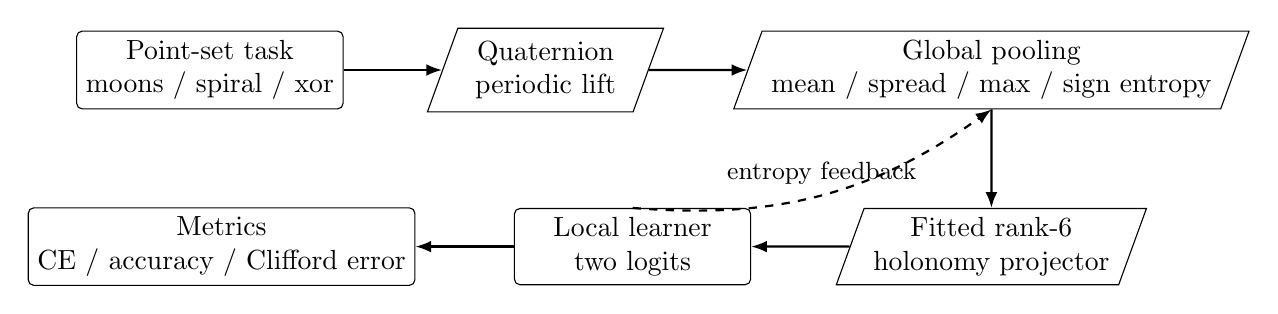
\begin{tikzpicture}[
  node distance=1.25cm,
  box/.style={draw, rounded corners=2pt, align=center, minimum width=3.0cm, minimum height=0.9cm},
  op/.style={draw, align=center, trapezium, trapezium left angle=70, trapezium right angle=110,
             minimum width=3.0cm, minimum height=0.9cm},
  arr/.style={-{Latex[length=2mm]}, thick}
]
\node[box] (data) {Point-set task\\moons / spiral / xor};
\node[op, right=of data] (lift) {Quaternion\\periodic lift};
\node[op, right=of lift] (pool) {Global pooling\\mean / spread / max / sign entropy};
\node[op, below=of pool] (proj) {Fitted rank-6\\holonomy projector};
\node[box, left=of proj] (learner) {Local learner\\two logits};
\node[box, left=of learner] (metrics) {Metrics\\CE / accuracy / Clifford error};

\draw[arr] (data) -- (lift);
\draw[arr] (lift) -- (pool);
\draw[arr] (pool) -- (proj);
\draw[arr] (proj) -- (learner);
\draw[arr] (learner) -- (metrics);
\draw[arr, dashed] (learner.north) to[bend right=20] node[above, font=\small] {entropy feedback} (pool.south);
\end{tikzpicture}
\end{center}

\section{Feature and Gate Definition}

The quaternion periodic feature lift emits seven channels per point:
\[
  [x,\ y,\ r,\ \mathrm{rotated}_x,\ \mathrm{rotated}_y,\ \mathrm{holonomy}_w,\ \mathrm{holonomy}_z].
\]

Global pooling produces four statistics per lifted channel:
\[
  \mathrm{mean},\quad \mathrm{spread},\quad \mathrm{max},\quad
  \mathrm{sign\ entropy}.
\]

The fitted projection gate estimates a rank-6 basis from class centroids and
rotor/holonomy channel groups, then applies alpha mixing:
\[
  \phi' = \alpha P(\phi) + (1-\alpha)\phi,\qquad \alpha=0.72.
\]

This is the key shift from scalar multiplication to projection. The gate shapes
the feature state by subspace selection instead of merely rescaling the update.

\section{Main Result}

The following table summarizes the fitted-projection extraction baseline. The
backprop-like timings come from the original HyMeKo workspace comparison; the
standalone extraction reproduces the local losses exactly after aligning rotor
conventions and pinning \texttt{rand = 0.9.2}.

\begin{center}
\begin{tabular}{lrrrrr}
\toprule
Task & Local acc & Local loss & Local \us/sample & Backprop-like \us/sample & Speedup\\
\midrule
moons  & 1.000 & 0.001513 & 5.673 & 139.984 & 24.7x\\
spiral & 1.000 & 0.004486 & 5.776 & 136.064 & 23.6x\\
xor    & 1.000 & 0.006714 & 4.178 & 136.299 & 32.6x\\
\bottomrule
\end{tabular}
\end{center}

The fitted projection stress learner reports 228 parameters. The original
backprop-like baseline reports 2836 parameters.

\section{Gate Ablation}

The difficult spiral few-shot/noisy/missing row is the most informative stress
case.

\begin{center}
\begin{tabular}{lrr}
\toprule
Gate & Accuracy & Loss\\
\midrule
Scalar entropy & 0.927 & 0.286730\\
Constant & 0.938 & 0.269849\\
Fixed projection & 0.906 & 0.324541\\
Fitted projection & 0.938 & 0.250603\\
\bottomrule
\end{tabular}
\end{center}

The fixed projector was algebraically closer to holonomy than scalar
multiplication, but it was too narrow. The fitted projector is the first version
that is both conceptually cleaner and empirically stronger on the hard row.

\section{Repository Layout}

\begin{center}
\begin{tabular}{>{\ttfamily}lp{0.58\linewidth}}
\toprule
Path & Purpose\\
\midrule
src/datasets.rs & Generated moons, spiral, xor data and corruption modes.\\
src/features.rs & Quaternion periodic lift using \texttt{hymeko\_clifford} rotors.\\
src/pooling.rs & Global mean/spread/max/sign-entropy pooling.\\
src/projection.rs & Fixed and fitted holonomy projection basis.\\
src/learner.rs & Local learner, gates, timing, stress ablation.\\
src/metrics.rs & Cross entropy and Clifford probability error.\\
examples/toy\_compare.rs & Reproducible toy benchmark.\\
reports/ & Raw JSON and markdown reports from the extraction.\\
\bottomrule
\end{tabular}
\end{center}

\section{Verification}

The current repository was verified with:

\begin{verbatim}
cargo test
cargo clippy --all-targets -- -D warnings
cargo run --release --example toy_compare -- \
  --tasks moons,spiral,xor --n-train 192 --n-test 96 \
  --n-points 32 --epochs 50 --batch-size 32 --lr 0.05 \
  --seed 53 --out reports/standalone-seed53-toy-run.json
\end{verbatim}

\section{Next Steps}

\begin{enumerate}
  \item Add explicit \texttt{project\_alpha\_mix\_forward} and
        \texttt{project\_alpha\_mix\_backward} kernels.
  \item Add finite-difference checks for projection gradients.
  \item Add a fixture parser for parity against the seed-53 run.
  \item Add graph/pgraph feature enrichment and structural generators.
  \item Compare against PyTorch CPU/GPU only at batch sizes where GPU overhead
        is meaningful.
\end{enumerate}

\section{Caveat}

The results are promising but narrow. Current evidence supports the statement
that projection-gated local holonomy learning is fast and compact on these
generated structured toy problems. It does not yet establish a general
replacement for backpropagation.

\end{document}
